% Compile with XeLaTeX, LuaLaTeX, or Tectonic.
% Required fonts: Times New Roman (text) and STIX Two Math (equations).
% Written directly from the strategy source code, not converted from a PDF.
\documentclass[11pt,letterpaper]{article}
\usepackage[margin=0.85in]{geometry}
\usepackage{fontspec}
\usepackage{amsmath}
\usepackage{unicode-math}
\usepackage{enumitem}
\usepackage{booktabs,tabularx,array}
\usepackage{microtype}
\usepackage{fancyhdr}
\usepackage{needspace}
\usepackage{tikz}
\usetikzlibrary{arrows.meta,positioning}
\usepackage[hidelinks]{hyperref}
\setmainfont{Times New Roman}
\setmathfont{STIX Two Math}
\setlength{\parindent}{0pt}
\setlength{\parskip}{5pt}
\setlist[itemize]{leftmargin=1.35em,itemsep=3pt,topsep=4pt,parsep=0pt}
\setlist[enumerate]{leftmargin=1.65em,itemsep=4pt,topsep=4pt,parsep=0pt}
\setlength{\emergencystretch}{1.5em}
\renewcommand{\arraystretch}{1.17}
\pagestyle{fancy}
\fancyhf{}
\fancyfoot[L]{\small Momentum Game Theory Strategy --- onboarding guide}
\fancyfoot[R]{\small\thepage}
\renewcommand{\headrulewidth}{0pt}
\renewcommand{\footrulewidth}{0.4pt}
\newcommand{\topic}[1]{\Needspace{5\baselineskip}\subsection*{#1}}
\newcommand{\word}[1]{\text{#1}}
\newcommand{\guidepage}[1]{\clearpage\section*{#1}}
\begin{document}

\begin{center}
{\LARGE\bfseries Momentum Game Theory Strategy}\\[4pt]
{\large A step-by-step onboarding guide}
\end{center}

\section*{1. Start with the idea}
\begin{itemize}
\item We use recent price performance to decide which groups of stocks to own. This is called \textbf{momentum}: assets that have performed strongly receive higher scores.
\item We also measure how similarly the investments move. The game-theory calculation reduces the attractiveness of sectors that duplicate exposure already in the portfolio.
\item The portfolio can move part or all of its money into Treasury bonds or cash when its equity rules fail.
\item We make these decisions \textbf{once each month}. This is a rule-based allocation process, with preset parameters.
\end{itemize}

\topic{Terms you need before reading the formulas}
\begin{itemize}
\item \textbf{ETF:} an exchange-traded fund, bought and sold like a stock. Each ETF here represents a group of stocks or Treasury bonds.
\item \textbf{Portfolio or book:} all of the strategy's investments and cash together.
\item \textbf{Sleeve:} one part of the portfolio with its own selection rules.
\item \textbf{Weight:} the fraction of money assigned to a holding. A 10\% weight in a \$100,000 portfolio means a \$10,000 investment.
\item \textbf{Rebalance:} buy or sell enough shares to move current holdings toward the newly calculated target weights.
\item \textbf{Defensive holding:} the Treasury ETF IEF or cash, selected using the rule explained on page~\pageref{style-rules}.
\end{itemize}

\topic{Two sleeves, with a fixed capital split}
\begin{itemize}
\item \textbf{65\% style sleeve:} normally holds one ETF representing a broad equity market or investment style.
\item \textbf{35\% sector sleeve:} normally holds four to six US sector ETFs, such as technology or healthcare.
\item Each sleeve can independently move its allocation to the defensive holding. The 65/35 split stays fixed; the assets receiving those allocations change.
\end{itemize}
\[
\word{Style capital}=0.65\times\word{Portfolio value}
\qquad
\word{Sector capital}=0.35\times\word{Portfolio value}
\]
\textbf{Example:} a \$100,000 portfolio assigns \$65,000 to the style rules and \$35,000 to the sector rules. In formulas, 65\% is written as 0.65.

\topic{The monthly sequence}
\begin{enumerate}
\item Calculate momentum scores and select the style holding.
\item Check whether the sector sleeve should own equities. If it should, rank sectors using momentum and the crowding calculation.
\item Turn the selections into portfolio weights, then into share orders.
\item Trade at the next trading day's close and hold until the next rebalance.
\end{enumerate}

\guidepage{2. What can we hold, and what data do we use?}
\topic{Style sleeve: seven candidates}
\begin{center}
\begin{tabularx}{0.95\linewidth}{@{}lX@{}}
\toprule
\textbf{Ticker} & \textbf{Exposure used by the strategy}\\
\midrule
SPY & Broad US large-company stocks\\
QQQ & Nasdaq-100 stocks\\
IWM & US small-company stocks\\
EFA & Developed international stocks\\
EEM & Emerging-market stocks\\
IWF & US large-company growth stocks\\
IWD & US large-company value stocks\\
\bottomrule
\end{tabularx}
\end{center}

\topic{Sector sleeve: eleven candidates}
\begin{center}
\begin{tabularx}{0.95\linewidth}{@{}lXlX@{}}
\toprule
\textbf{Ticker} & \textbf{Sector label} & \textbf{Ticker} & \textbf{Sector label}\\
\midrule
IYW & Technology & IYF & Financials\\
IYH & Healthcare & IYE & Energy\\
IYC & Consumer discretionary & IYZ & Telecommunications\\
IYK & Consumer staples & IDU & Utilities\\
IYM & Materials & IYJ & Industrials\\
IYR & Real estate & & \\
\bottomrule
\end{tabularx}
\end{center}

\topic{Defensive choices}
\begin{itemize}
\item \textbf{IEF:} an ETF holding US Treasury bonds with maturities of roughly seven to ten years. Its price can fall, so it must pass its own return test.
\item \textbf{Cash:} money left uninvested. The backtest models a T-bill return on this balance; the broker's actual cash interest can differ.
\end{itemize}

\topic{Inputs to the calculations}
\begin{itemize}
\item \textbf{Adjusted ETF prices} come from yfinance and account for distributions and splits. Final trading prices each month drive momentum and return hurdles; daily returns drive correlations and the optional volatility control.
\item \textbf{The three-month US T-bill yield} comes from FRED's DGS3MO series. The code converts this annualized yield into an estimated cash return.
\item An ETF needs enough history to calculate all three momentum horizons and skip the most recent month. Missing scores are excluded from ranking.
\item A usable signal requires a completed month and available T-bill comparison data. A partial month's return is not a valid monthly signal.
\end{itemize}

\guidepage{3. Momentum: turn price changes into a ranking}
\topic{Step 1: calculate a return}
A return measures how much an adjusted price changed over a chosen period:
\[
\word{Return}=\frac{\word{Ending adjusted price}}{\word{Starting adjusted price}}-1.
\]
\begin{itemize}
\item If the price moves from 100 to 112, the return is $112/100-1=0.12$, or \textbf{12\%}.
\item For ranking, we calculate \textbf{three-, six-, and twelve-month returns}, each ending one month before the signal month-end.
\item Example: for a September month-end signal, the three-month ranking return uses June, July, and August. It compares the end-of-May price with the end-of-August price. September is skipped.
\end{itemize}

\topic{Step 2: put the three horizons on a comparable scale}
A raw twelve-month return can have a different typical size and spread from a three-month return. We standardize each horizon before averaging it:
\[
\word{Standardized score}
=\frac{\word{ETF's return}-\word{Average return of its group}}
{\word{Standard deviation of returns in its group}}.
\]
\begin{itemize}
\item A \textbf{standard deviation} measures spread. Here it describes how widely the ETFs' returns differ from one another at a given horizon.
\item The code uses the sample standard deviation. The style candidates form one comparison group; the sector candidates form another.
\item This standardized score is also called a \textbf{z-score}. A score of 0 means average performance; +1 means one standard deviation above average; negative means below average.
\end{itemize}
\textbf{Example:} if an ETF returned 12\%, its group averaged 8\%, and the group's standard deviation was 4 percentage points:
\[
\word{Standardized score}=\frac{12\%-8\%}{4\%}=1.
\]

\topic{Step 3: average the three standardized scores}
\[
\word{Momentum score}
=\frac{\word{3-month score}+\word{6-month score}+\word{12-month score}}{3}.
\]
\begin{itemize}
\item If the scores are 1.0, 0.5, and 1.5, the momentum score is $(1.0+0.5+1.5)/3=1.0$.
\item Higher scores mean stronger performance relative to peers across these horizons. A score of 1.0 is a ranking value, not a forecast of a 1\% return.
\item Relative strength alone does not show that prices rose: an ETF can rank first while losing money. The style sleeve therefore has an additional cash-return hurdle.
\end{itemize}

\guidepage{4. Choose the style holding and the defensive holding}
\label{style-rules}
\topic{The cash-return hurdle}
\begin{itemize}
\item A style ETF passes if its latest \textbf{six-month return beats six-month cash}, or its latest \textbf{twelve-month return beats twelve-month cash}. Passing either test is enough.
\item These returns \textbf{include the signal month}. For a September signal, the six-month hurdle uses April through September. This differs from the momentum ranking, which skips September.
\item The six-month test lets an ETF qualify during a recovery before its twelve-month return has caught up.
\end{itemize}
\[
\begin{aligned}
\word{Pass if:}\quad&\word{ETF 6-month return}>\word{Cash 6-month return}\\
&\word{OR}\\
&\word{ETF 12-month return}>\word{Cash 12-month return}.
\end{aligned}
\]
\textbf{Example:} an ETF with a six-month return of 8\% passes against 2\% cash even if its twelve-month return of $-3\%$ fails against 4\% cash.

\topic{How the code makes the style selection}
\begin{enumerate}
\item Rank the seven candidates by momentum score.
\item If the first-ranked ETF passes the hurdle, assign the entire style sleeve to it.
\item If it fails, keep the previous style ETF only if that ETF is still in the top two and passes the hurdle.
\item Otherwise assign the entire style sleeve to the defensive holding.
\end{enumerate}
\begin{itemize}
\item A qualifying new leader replaces a second-ranked incumbent. The current code does not keep the second-ranked ETF merely because it remains in the top two.
\item It also does not search further down the ranking for a different passing ETF. A lower-ranked ETF can pass the hurdle while the sleeve still becomes defensive.
\end{itemize}

\topic{The defensive rule used by either sleeve}
\begin{itemize}
\item Choose \textbf{IEF} only if its latest twelve-month return is greater than the twelve-month cash return. Otherwise choose \textbf{cash}.
\item IEF uses the twelve-month test only. It cannot qualify through the six-month test.
\item If both sleeves become defensive, their allocations combine into 100\% IEF or 100\% cash, according to this same rule.
\end{itemize}

\topic{How the cash comparison is estimated}
\begin{itemize}
\item The code estimates each month's cash return from the previous month's annualized T-bill yield divided by 12. For example, 4.8\% per year gives roughly 0.4\% for a month.
\item It compounds six or twelve monthly estimates: multiply each month's $(1+\word{return})$, then subtract 1. Six months at 0.4\% gives $1.004^6-1\approx2.42\%$.
\end{itemize}

\guidepage{5. From the style decision to the sector candidates}
\label{sector-overlap}
The style sleeve has now chosen its holding. We make a separate decision for the 35\% sector sleeve. The style holding matters here because we want the sector picks to account for investments already in the other 65\% of the portfolio.

\topic{Start with each sector's original momentum score}
\begin{itemize}
\item Use the same momentum method as the style sleeve: calculate three-, six-, and twelve-month returns, each \textbf{ending before the newest month}. A September signal's three-month ranking return, for example, uses the change from the end of May to the end of August:
\end{itemize}
\[
\word{Three-month return}
=\frac{\word{Adjusted price at end of August}}
{\word{Adjusted price at end of May}}-1.
\]
For each horizon, compare a sector's return with the returns of the other \textbf{scoreable sector ETFs}. The average and standard deviation come from that sector group, which can contain up to eleven ETFs:
\[
\word{Three-month standardized score}
=\frac{\word{Sector's three-month return}-\word{Group's average three-month return}}
{\word{Group's sample standard deviation}}.
\]
Calculate the six- and twelve-month standardized scores the same way, using a separate group average and spread at each horizon. Then:
\[
\word{Original sector momentum score}
=\frac{\word{3-month score}+\word{6-month score}+\word{12-month score}}{3}.
\]
\begin{itemize}
\item The score compares \textbf{sectors with sectors}; the seven style ETFs form a different group. A score of 1.2 is a ranking number, not a 1.2\% return.
\item Sectors have no individual T-bill hurdle. Taking the four highest original scores could repeat the same market exposure, so the game adjusts their ranking for overlap.
\end{itemize}

\topic{Check whether the sector sleeve can hold equities}
A \textbf{moving average} is the average of recent daily closing prices. The rule depends on whether the sector sleeve was holding equities or was defensive last month:
\begin{itemize}
\item \textbf{Currently in sectors:} leave equities if SPY ends the month at or below its \textbf{231-day} average.
\item \textbf{Currently defensive:} return to sectors if SPY ends the month above its \textbf{63-day} average.
\item A defensive month puts all 35\% in IEF or cash and clears the old sector holdings. The game runs only when the sleeve is allowed to own sectors.
\end{itemize}

\guidepage{6. How correlation and crowding are calculated}
\topic{Which ETFs are compared?}
\begin{itemize}
\item Pick one candidate sector, such as IYW. Compare its daily returns separately with \textbf{each scoreable sector ETF}, including IYW itself. When all eleven have scores, that is ten other sector comparisons plus one self-comparison.
\item Also compare IYW with the \textbf{one asset already selected by the style sleeve}, such as QQQ. The code does not compare it with all seven possible style ETFs. If the style sleeve holds IEF, compare it with IEF; if it holds cash, there is no style-price correlation to calculate.
\item Repeat this for each candidate sector. The same monthly calculation produces a table of sector-to-sector and sector-to-style correlations.
\end{itemize}

\topic{Calculate each pair's correlation}
The code takes the latest \textbf{126 daily return rows} available at month-end. For each ETF on each day:
\[
\word{Daily return}=\frac{\word{Today's adjusted close}}{\word{Yesterday's adjusted close}}-1.
\]
For a pair A and B, line up returns from the same dates. Let $A_d$ and $B_d$ be their returns on day $d$; let $\overline A$ and $\overline B$ be the average of each ETF's paired daily returns; and let $N$ be the number of valid paired days. The calculation is:
\[
\begin{aligned}
\word{Covariance}(A,B)&=\frac{\sum_{d=1}^{N}(A_d-\overline A)(B_d-\overline B)}{N-1},\\[4pt]
\word{Correlation}(A,B)&=\frac{\word{Covariance}(A,B)}
{\word{Standard deviation}(A)\times\word{Standard deviation}(B)}.
\end{aligned}
\]
\begin{itemize}
\item This is Pearson correlation. It is near +1 when returns usually rise and fall together, near 0 when there is little linear relationship, and near $-1$ when they usually move in opposite directions.
\item The self-correlation is set to 1. If a pair's correlation cannot be calculated from available prices, the code uses 0 for that pair. Correlations are held fixed during the month's 300 game rounds.
\end{itemize}

\topic{Turn correlations into crowding exposure}
The game assigns each sector a temporary \textbf{game weight}. These weights start equally and always add to 35\% of the portfolio. For one candidate sector, add two contributions:
\[
\begin{aligned}
\word{Sector contribution}&=\word{sum over all sectors of}\;(
\word{game weight}\times\word{correlation with candidate}),\\
\word{Style contribution}&=0.65\times\word{correlation with selected style holding},\\
\word{Total crowding exposure}&=\word{Sector contribution}+\word{Style contribution}.
\end{aligned}
\]
The sector contribution includes the candidate's own game weight because its self-correlation is 1. For example, a sector whose correlation with the selected style ETF is 0.80 gets a style contribution of $0.65\times0.80=0.52$. If the style holding is cash, its contribution is zero. Negative correlations reduce the crowding total.

\guidepage{7. The congestion game: fixed inputs and changing weights}
The sector ETFs compete for a fixed 35\% pool of \textbf{temporary game weight}. This is a way to rank them: a sector with strong momentum can lose ground when it overlaps heavily with the other investments. The selected style ETF has already received its 65\% allocation, so its effect on each sector is known before the game starts.

\topic{What stays the same during one month's 300 rounds?}
\begin{center}
\begin{tabularx}{\linewidth}{@{}>{\bfseries\raggedright\arraybackslash}p{0.39\linewidth}X@{}}
\toprule
Fixed for all 300 rounds & Recalculated in every round\\
\midrule
Each sector's original momentum score & Each sector's sector contribution to crowding, from the current game weights\\
The sector correlation matrix from the last 126 daily return rows & Each sector's total crowding exposure (sector plus style)\\
The chosen style ETF and its 65\% allocation & Each sector's adjusted score, called its payoff\\
Each sector's style contribution: $0.65\times\word{correlation with style ETF}$ & Each sector's temporary game weight after the update\\
The sector sleeve's 35\% total & The split of that 35\% among the sectors\\
\bottomrule
\end{tabularx}
\end{center}
\textbf{Key distinction:} the style contribution does not change within the game. The sector contribution changes because the temporary weights change. A new monthly signal calculates new inputs and starts a new 300-round game.

\topic{Follow one round, then feed its weights into the next}
\begin{center}
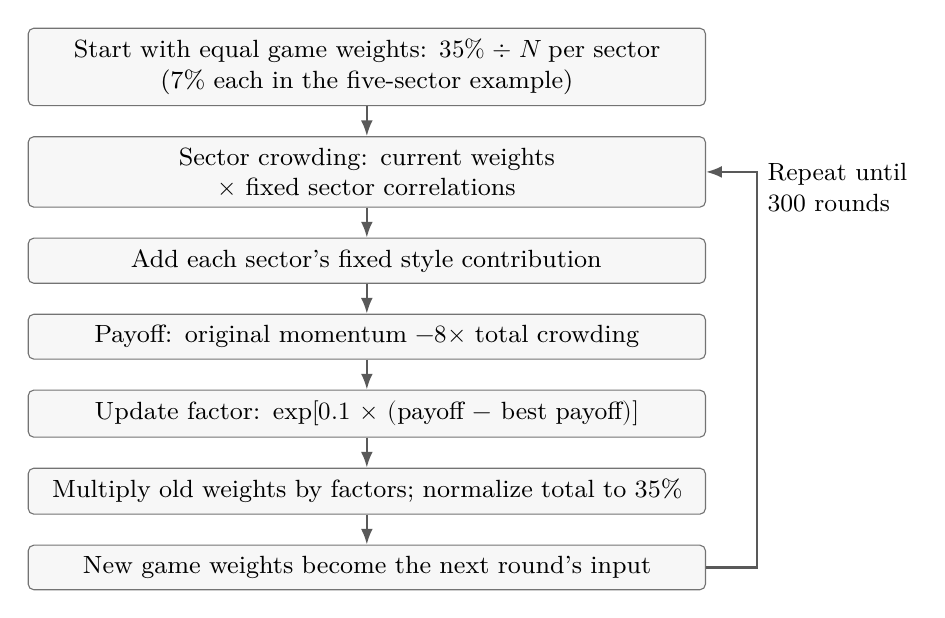
\begin{tikzpicture}[
  box/.style={draw=black!55,rounded corners=2pt,fill=black!3,
    text width=0.69\linewidth,align=center,inner ysep=4pt,font=\small},
  flow/.style={-{Latex[length=2mm]},thick,draw=black!65},
  node distance=3.8mm]
\node[box] (a) {Start with equal game weights: $35\%\div N$ per sector\\(7\% each in the five-sector example)};
\node[box,below=of a] (b) {Sector crowding: current weights $\times$ fixed sector correlations};
\node[box,below=of b] (c) {Add each sector's fixed style contribution};
\node[box,below=of c] (d) {Payoff: original momentum $-8\times$ total crowding};
\node[box,below=of d] (e) {Update factor: $\exp[0.1\times(\word{payoff}-\word{best payoff})]$};
\node[box,below=of e] (f) {Multiply old weights by factors; normalize total to 35\%};
\node[box,below=of f] (g) {New game weights become the next round's input};
\foreach \x/\y in {a/b,b/c,c/d,d/e,e/f,f/g}{\draw[flow] (\x)--(\y);}
\draw[flow] (g.east) -- ++(0.65,0) |- (b.east)
  node[pos=0.48,right,font=\small,align=left] {Repeat until\\300 rounds};
\end{tikzpicture}
\end{center}

With all eleven real sectors available, each starts at $35\%/11\approx3.18\%$. The example on the next pages uses five sectors so every step fits on the page; each starts at $35\%/5=7\%$.

\guidepage{8. Five-sector example: inputs and Round 1}
\textbf{Hypothetical monthly inputs.} Suppose the style sleeve chose SPY at 65\%. We use five sectors to show the arithmetic. The original momentum scores come from the method on page 5 and stay fixed for the whole example. Correlations also stay fixed.
\begin{center}
\begin{tabular}{@{}lrrr@{}}
\toprule
Sector & Original momentum & Correlation with SPY & Starting game weight\\
\midrule
Technology & 1.20 & 0.70 & 7.00\%\\
Financials & 0.80 & 0.40 & 7.00\%\\
Healthcare & 0.40 & 0.10 & 7.00\%\\
Energy & $-0.30$ & 0.10 & 7.00\%\\
Industrials & $-1.10$ & 0.30 & 7.00\%\\
\bottomrule
\end{tabular}
\end{center}
\textbf{Sector-to-sector correlations:} read across a row to see how that sector moves with each column. A sector's correlation with itself is 1.
\begin{center}
\begin{tabular}{@{}lrrrrr@{}}
\toprule
 & Technology & Financials & Healthcare & Energy & Industrials\\
\midrule
Technology & 1.00 & 0.60 & 0.20 & 0.10 & 0.50\\
Financials & 0.60 & 1.00 & 0.20 & 0.30 & 0.50\\
Healthcare & 0.20 & 0.20 & 1.00 & 0.10 & 0.20\\
Energy & 0.10 & 0.30 & 0.10 & 1.00 & 0.40\\
Industrials & 0.50 & 0.50 & 0.20 & 0.40 & 1.00\\
\bottomrule
\end{tabular}
\end{center}

\topic{Round 1, steps 1--4: calculate all five payoffs}
First calculate the fixed style contribution: for Technology, $0.65\times0.70=0.455$. Next multiply the \emph{Technology row} of the matrix by the starting sector weights and add the five products:
\[
\word{Technology sector crowding}=1(0.07)+0.60(0.07)+0.20(0.07)+0.10(0.07)+0.50(0.07)=0.168.
\]
Then add style crowding, $0.168+0.455=0.623$, and calculate Technology's payoff: $1.20-8(0.623)=-3.784$. Do the same for every row:
\begin{center}
\small
\begin{tabular}{@{}lrrrrr@{}}
\toprule
Sector & Momentum & Style crowding & Sector crowding & Total crowding & Payoff\\
\midrule
Technology & 1.200 & 0.455 & 0.168 & 0.623 & $-3.784$\\
Financials & 0.800 & 0.260 & 0.182 & 0.442 & $-2.736$\\
Healthcare & 0.400 & 0.065 & 0.119 & 0.184 & $-1.072$\\
Energy & $-0.300$ & 0.065 & 0.133 & 0.198 & $-1.884$\\
Industrials & $-1.100$ & 0.195 & 0.182 & 0.377 & $-4.116$\\
\bottomrule
\end{tabular}
\end{center}
Healthcare has the \textbf{best payoff in Round 1}: $-1.072$ is the highest value. Payoffs are relative ranking scores, so a negative value is valid. The fixed \textbf{8} is the code's crowding coefficient \texttt{GAME\_LAM}; it scales crowding into score points. A 0.10 crowding difference changes a payoff by 0.80 points, holding momentum equal. The repository does not document a derivation for exactly 8.

\guidepage{9. Five-sector example: finish Round 1}
\topic{Steps 5--8: find the best payoff, update, and normalize}
The \textbf{best payoff} in the formula is Healthcare's $-1.072$; each sector uses \emph{its own} payoff in the other slot. The code computes:
\[
\begin{aligned}
\word{Update factor}&=\exp\{0.1(\word{sector payoff}-\word{best payoff})\},\\
\word{Provisional weight}&=\word{old game weight}\times\word{update factor},\\
\word{New game weight}&=35\%\times
\frac{\word{provisional weight}}{\word{sum of five provisional weights}}.
\end{aligned}
\]
Here $\exp(x)=e^x$ and $e\approx2.718$. For Technology the factor is $\exp[0.1(-3.784-(-1.072))]=0.762464$; its provisional weight is $7\%\times0.762464\approx5.337248\%$.
\begin{center}
\small
\begin{tabular}{@{}lrrrr@{}}
\toprule
Sector & Old weight & Update factor & Provisional weight & New weight\\
\midrule
Technology & 7.000000\% & 0.762464 & 5.337248\% & 6.251540\%\\
Financials & 7.000000\% & 0.846707 & 5.926952\% & 6.942263\%\\
Healthcare & 7.000000\% & 1.000000 & 7.000000\% & 8.199128\%\\
Energy & 7.000000\% & 0.922009 & 6.454065\% & 7.559672\%\\
Industrials & 7.000000\% & 0.737566 & 5.162961\% & 6.047396\%\\
\midrule
Total & 35.000000\% & & 29.881226\% & 35.000000\%\\
\bottomrule
\end{tabular}
\end{center}
For example, Technology's new weight is $35\%\times(5.337248\%/29.881226\%)\approx6.251540\%$. The sum returns to 35\%. The \textbf{0.1} is the update speed: a payoff one point below the best receives factor $e^{-0.1}\approx0.905$. Small rounding differences in printed tables are possible.

\topic{Why did the best sector gain weight if its factor is only 1?}
Healthcare's payoff is the best in this round, so its update factor is $\exp(0)=1$. Its provisional weight stays at 7\%. The other sectors receive factors below 1, shrinking the total of all provisional weights to 29.881226\%. Normalization then scales \emph{all} five provisional weights up by $35\%/29.881226\%\approx1.171304$. Healthcare therefore ends at $7\%\times1.171304\approx8.199128\%$. The formula compares each sector with the \textbf{best payoff in the same round}; Round 2 will find a new best payoff.

\guidepage{10. Five-sector example: Round 2}
Now use the five \textbf{new weights from Round 1} as the starting weights. Momentum scores, the correlation matrix, and style contributions are exactly the same. Sector crowding must be calculated again because the weight on each sector changed.

\topic{Round 2, steps 1--4: recalculate crowding and payoffs}
The Technology row now uses the updated weights, written as fractions of the full portfolio:
\[
\begin{aligned}
\word{Technology sector crowding}={}&1(0.062515400)+0.60(0.069422632)\\
&+0.20(0.081991282)+0.10(0.075596722)+0.50(0.060473964)\\
\approx{}&0.158364.
\end{aligned}
\]
Its \textbf{style crowding remains 0.455}. Thus its new total crowding is about $0.158364+0.455=0.613364$, and its new payoff is $1.20-8(0.613364)\approx-3.706911$. All five recalculations are:
\begin{center}
\small
\begin{tabular}{@{}lrrrrr@{}}
\toprule
Sector & Momentum & Style crowding & Sector crowding & Total crowding & Payoff\\
\midrule
Technology & 1.200 & 0.455 & 0.158364 & 0.613364 & $-3.706911$\\
Financials & 0.800 & 0.260 & 0.176246 & 0.436246 & $-2.689969$\\
Healthcare & 0.400 & 0.065 & 0.128033 & 0.193033 & $-1.144267$\\
Energy & $-0.300$ & 0.065 & 0.135064 & 0.200064 & $-1.900510$\\
Industrials & $-1.100$ & 0.195 & 0.173080 & 0.368080 & $-4.044639$\\
\bottomrule
\end{tabular}
\end{center}
Healthcare remains the best payoff in Round 2, but the best value has changed to $-1.144267$. Use \textbf{this round's best payoff} when calculating every Round 2 factor.

\topic{Round 2, steps 5--8: update and normalize again}
For Technology, the factor is $\exp[0.1(-3.706911-(-1.144267))]\approx0.773937$. Multiply its \emph{Round 1 ending weight} by this factor: $6.251540\%\times0.773937\approx4.838300\%$ provisional weight. Repeat for every sector:
\begin{center}
\small
\begin{tabular}{@{}lrrrr@{}}
\toprule
Sector & Old weight & Update factor & Provisional weight & New weight\\
\midrule
Technology & 6.251540\% & 0.773937 & 4.838300\% & 5.548622\%\\
Financials & 6.942263\% & 0.856783 & 5.948015\% & 6.821257\%\\
Healthcare & 8.199128\% & 1.000000 & 8.199128\% & 9.402861\%\\
Energy & 7.559672\% & 0.927164 & 7.009059\% & 8.038075\%\\
Industrials & 6.047396\% & 0.748236 & 4.524878\% & 5.189185\%\\
\midrule
Total & 35.000000\% & & 30.519381\% & 35.000000\%\\
\bottomrule
\end{tabular}
\end{center}
Technology's normalized weight is $35\%\times(4.838300\%/30.519381\%)\approx5.548622\%$. Each new weight is the input to the next round. The code repeats this same sequence \textbf{300 times in total}; it uses the weights after Round 300 for ranking. It does not wait for exact convergence.

\guidepage{11. Compare the two rounds}
\topic{What changed between the two rounds?}
In this table, ``game weight'' means the weight \emph{after} that round's update. The corresponding crowding and payoff were calculated \emph{before} that update.
\begin{center}
\small
\begin{tabular}{@{}lrrrrrr@{}}
\toprule
& \multicolumn{2}{c}{Total crowding} & \multicolumn{2}{c}{Payoff} & \multicolumn{2}{c}{Ending game weight}\\
\cmidrule(lr){2-3}\cmidrule(lr){4-5}\cmidrule(l){6-7}
Sector & Round 1 & Round 2 & Round 1 & Round 2 & Round 1 & Round 2\\
\midrule
Technology & 0.623000 & 0.613364 & $-3.784000$ & $-3.706911$ & 6.2515\% & 5.5486\%\\
Financials & 0.442000 & 0.436246 & $-2.736000$ & $-2.689969$ & 6.9423\% & 6.8213\%\\
Healthcare & 0.184000 & 0.193033 & $-1.072000$ & $-1.144267$ & 8.1991\% & 9.4029\%\\
Energy & 0.198000 & 0.200064 & $-1.884000$ & $-1.900510$ & 7.5597\% & 8.0381\%\\
Industrials & 0.377000 & 0.368080 & $-4.116000$ & $-4.044639$ & 6.0474\% & 5.1892\%\\
\bottomrule
\end{tabular}
\end{center}
This is the feedback loop: \textbf{changing game weights $\rightarrow$ changing sector crowding $\rightarrow$ changing payoffs $\rightarrow$ changing game weights}. For example, Healthcare's game weight rose after Round 1, so its own sector crowding increased in Round 2. Its style crowding stayed at 0.065. Although Technology began with the strongest momentum, its large overlap with SPY reduced its payoff. That is how the game balances momentum against duplicate exposure.

\textbf{What the loop teaches:} a higher game weight can raise a sector's own crowding next round; a lower game weight can relieve it. The original momentum scores and style overlap do not move during these rounds. The game therefore keeps reconsidering which sectors offer strong momentum without concentrating too much of the same exposure.

\topic{Read the change in two specific rows}
\begin{itemize}
\item \textbf{Technology:} its sector crowding falls from 0.168000 to about 0.158364 because the sector weights changed. Its style crowding stays 0.455. The 0.009636 fall in total crowding improves its payoff by about $8\times0.009636=0.077088$ points. Its game weight still falls because the other sectors' relative payoffs are better.
\item \textbf{Healthcare:} its sector crowding rises from 0.119000 to about 0.128033. Its style crowding stays 0.065, so its payoff gets about 0.072267 points worse. It remains the best payoff in Round 2 and, after normalization, its game weight rises again.
\end{itemize}

\guidepage{12. After Round 300: choose and size holdings}
\topic{Use game weights to rank sectors}
The temporary game weights have now served their purpose. The code ranks the sectors by their \textbf{final game weights}; those percentages do \textbf{not} become actual portfolio position sizes.
\begin{enumerate}
\item Include sectors ranked in the top four by the final game weights.
\item Also keep previously held sectors that are still ranked in the top six.
\item Remove previous holdings that have fallen below sixth place.
\item Split the sector sleeve equally across the resulting set.
\end{enumerate}
\begin{itemize}
\item \textbf{Sizing example:} suppose four selected sectors finish the game at 12\%, 9\%, 8\%, and 6\% temporary weight. Each actual holding receives $35\%/4=8.75\%$ of the portfolio; we do not invest 12\%, 9\%, 8\%, and 6\%.
\item \textbf{Retention example:} last month we held A, B, C, and D. This month's ranking is A, B, E, F, C, D. The new top four are A, B, E, and F; C and D also remain because they rank fifth and sixth. The six actual holdings each receive about 5.83\%.
\item This retention rule can reduce trading. Exact ranking ties follow the code's average-rank convention.
\end{itemize}

\topic{Calculate the actual portfolio weights}
\[
\word{Weight of each selected sector}
=\frac{35\%}{\word{Number of selected sectors}}.
\]
\begin{center}
\begin{tabular}{@{}ccc@{}}
\toprule
\textbf{Sectors held} & \textbf{Weight per sector} & \textbf{Total sector allocation}\\
\midrule
4 & 8.75\% & 35\%\\
5 & 7.00\% & 35\%\\
6 & About 5.83\% & 35\%\\
\bottomrule
\end{tabular}
\end{center}
The style sleeve gives its chosen asset 65\% of the book. More generally, for any asset:
\[
\begin{aligned}
\word{Total portfolio weight}={}&0.65\times\word{Fraction of style sleeve in that asset}\\
&+0.35\times\word{Fraction of sector sleeve in that asset}.
\end{aligned}
\]
\textbf{Example:} if SPY is the style selection and there are four sector selections, a \$100,000 model portfolio holds \$65,000 SPY and \$8,750 in each sector. If sectors become defensive, their \$35,000 moves to IEF or cash.

\guidepage{13. Operating the strategy}
\topic{Convert weights into share orders}
\[
\word{Target shares}\approx
\frac{\word{Portfolio weight}\times\word{Investable account value in USD}}
{\word{Latest ETF share price}}.
\]
\begin{itemize}
\item The execution code holds back \textbf{0.5\% of account value} as a cash buffer, then rounds target shares to whole shares. A \$100,000 account therefore starts with \$99,500 for sizing.
\item A sector with an 8.75\% target and a \$100 price would receive about $0.0875\times99{,}500/100=87.06$, rounded to 87 shares.
\item Order size equals target shares minus shares already held. Actual weights can differ because of rounding, funding adjustments, price moves, and the closing-auction fill price.
\end{itemize}

\topic{Monthly operating checklist}
\begin{enumerate}
\item \textbf{Refresh and check the signal.} After the completed month-end, refresh price and T-bill data. Confirm the reported signal date and inspect the target holdings.
\item \textbf{Review the dry run.} The execution program compares targets with broker positions and prints proposed buys and sells. Account values must be expressed in USD for sizing these ETFs.
\item \textbf{Check funding.} The execution code checks USD cash and sale proceeds, and can scale down buys when estimated funding is insufficient. The cash buffer reduces the chance of borrowing but cannot remove uncertainty in the eventual fill prices.
\item \textbf{Execute the rebalance.} Orders are intended for the next trading day's closing auction. The broker connection defaults to a paper-account check; transmitting orders requires the execution mode and its confirmation.
\item \textbf{Confirm fills and holdings.} Check the completed orders and resulting positions. Between monthly rebalances, market moves cause the weights to drift.
\end{enumerate}

\topic{The optional volatility throttle is currently off}
\begin{itemize}
\item \textbf{Volatility} means the variability of returns. The current setting is \texttt{BOOK\_VT = 0}, so this control makes no changes to the portfolio.
\item If a positive volatility cap is enabled, the control can act when SPY is at or below its 126-day average. It estimates annualized volatility using the target holdings and the last 21 daily returns.
\item If measured volatility exceeds the chosen cap, it scales equity positions down by the ratio below and transfers the released money to the defensive holding:
\end{itemize}
\[
\word{Scale factor}=\frac{\word{Volatility cap}}{\word{Measured annualized volatility}}.
\]
\textbf{Example:} a 15\% cap against 20\% measured volatility gives a factor of 0.75. The control would retain 75\% of each equity position. It does not increase exposure when volatility is below the cap.

\vfill
{\footnotesize\textbf{Source and reproducibility.} Rules are based on \path{strategy/strategy_lib.py} and share sizing on \path{strategy/live/execute_rebalance.py}. The detailed mathematical reference is \path{docs/Strategy_Mathematical_Formulation.md}. All numerical examples in this guide are illustrations, not current trading signals.}

\end{document}
